\subsection{Componente per il mapping}
La prima componente che si descrive è quella relativa
al mapping tra una colonna e la sua successiva nella matrice $\PBWT$. Bisogna 
studiare come effettuare il forward-step/mapping nella $\RLPBWT$ e
memorizzare, per 
ogni colonna $k$ e in modo proporzionale al numero di run della stessa, le
informazioni necessarie a ottenere i medesimi risultati della funzione
$w(i,\sigma)$ (secondo la notazione di Durbin). 
\subsubsection{Mapping con intvector compressi}
La prima variante che si descrive è quella denominata \texttt{MAP-INT}.\\
L'ispirazione iniziale per tale componente è stata data dall'articolo di Gagie
et al \cite{tricks}. Riprendendo quanto descritto al termine della sezione
\ref{secpbwt}, si è deciso di
memorizzare gli indici delle teste di run, ma quest'informazione non è
sufficiente per poter sapere 
se una run sia composta da simboli $\sigma=0$ o simboli
$\sigma=1$. Essendo lo studio limitato a pannelli costruiti su alfabeto binario
$\Sigma=\{0,1\}$, si è 
potuto sfruttare il fatto che le run si alternino tra un carattere e
l'altro. Basta quindi tenere in memoria un valore booleano nominato
$start_k$, che permetta di 
capire se, in colonna $k$, la prima run sia costituita da simboli
$\sigma=0$. Le run di 
indice pari presentano lo stesso simbolo della prima run e quindi, dato un
qualsiasi indice di run, è possibile sapere quale sia il simbolo corrispondente.
L'implementazione di questo concetto si ritrova nella
funzione $\GS$, la quale è
visualizzabile all'algoritmo \ref{algo:extrchar} e richiede tempo costante.
\begin{algorithm}
  \footnotesize
  \begin{algorithmic}[1]
    \Function{get\_symbol}{$k, \,\,r$}
    \Comment $k$ indice di colonna, $r$ indice di run
    \If{$start_k$}
    \State \textbf{if} $r\bmod 2 = 0$ \textbf{then} \textbf{return} $0$
    \textbf{else} \textbf{return} $1$
    \Else
    \State \textbf{if} $r\bmod 2 = 0$ \textbf{then} \textbf{return} $1$
    \textbf{else} \textbf{return} $0$
    \EndIf
    \EndFunction
  \end{algorithmic}
  \caption{Algoritmo per estrazione simbolo da una run in una colonna.}
  \label{algo:extrchar}
\end{algorithm}

Si memorizzano gli indici delle teste di run in un array $p_k$, di lunghezza
pari al numero di run in colonna $k$, avendo che un indice $i\in\{0,M-1\}$ è
una testa di run sse: 
\begin{equation}
  \label{eq:naive1}
  i=0\lor y_{i-1}^k[k]\neq y_i^k[k]
\end{equation}
Il passaggio successivo è stato quello di capire se le informazioni memorizzate
per il mapping siano tutte necessarie, ovvero se, data la colonna $k$
nella matrice $\PBWT$, siano necessari interamente $c[k]$, $u_k$ e $v_k$. In
merito al valore $c[k]$, si è deciso che si possa calcolarlo 
in fase di costruzione delle $\RLPBWT$ e memorizzarlo esattamente come per
la $\PBWT$, avendo in totale $N$ valori per l'intera trasformata. In merito,
invece, ai vettori $u_k$ e $v_k$ si è cercato un modo 
per ottenerne una rappresentazione che implichi memorizzare un solo valore per
ogni 
run della colonna. In altri termini, si è cercato di capire se sia possibile
tenere in memoria $r$ valori (con $r$ numero di run in una colonna) che
permettano di effettuare comunque il 
mapping, a partire da un indice arbitrario $i\in\{0,\ldots,M-1\}$. L'alternanza
data dal caso binario ha permesso di trovare una 
semplice soluzione, avendo che i valori di $u_k$ e $v_k$ crescono in
modo 
alternato. Infatti, a seconda del simbolo $\sigma$ rappresentato in una data
run, si ha che solo i valori dell'array relativo a tale simbolo, nel range di
indici di quella run, verranno incrementati, a ogni passo, di un'unità. Facendo
un esempio, se in una run di simboli $\sigma=0$ si itera
virtualmente all'interno di tale run, solo i valori di $u_k$, in quel
range di indici, cresceranno di volta in volta di uno mentre per $v_k$, nello
stesso range, si avrà sempre lo stesso valore.
\begin{esempio}
  Data la seguente colonna:
  \[y^5=00101111000000000000\]
  si hanno, oltre a $c[5]=15$:
  \begin{table}[H]
    \footnotesize
    \centering
    \begin{tabular}{c||cc|c|c|cccc|cccccccccccc}
      & 0 & 1 & 2 & 3 & 4 & 5 & 6 & 7 & 8 & 9 & 10 & 11 & 12 & 13 & 14 & 15 & 16
      & 17 & 18 & 19\\
      \hline
      \hline
      $y^5$ & 0 & 0 & 1 & 0 & 1 & 1 & 1 & 1 & 0 & 0 & 0 & 0 & 0 & 0 & 0 & 0 & 0
      & 0 & 0 & 0\\
      \hline
      \hline
      $u_5$ & 0 & 1 & 2 & 2 & 3 & 3 & 3 & 3 & 3 & 4 & 5 & 6 & 7 & 8 & 9 & 10
      & 11 & 12 & 13 & 14\\
      \hline
      $v_5$ & 0 & 0 & 0 & 1 & 1 & 2 & 3 & 4 & 5 & 5 & 5 & 5 & 5 & 5 & 5 & 5 & 5
      & 5 & 5 & 5
    \end{tabular}
  \end{table}
  \noindent
  Dove si nota l'alternanza di crescita dei valori, come sopra descritto.
\end{esempio}
Grazie a questo comportamento, è possibile memorizzare, per ogni indice di
testa di run $i$, tale che $i\neq 0$, solo il valore di $u_k[i]$ o $v_k[i]$,
rispettivamente se sia una run su simboli $\sigma=1$ o $\sigma=0$.
Per $i=0$ si ha $u_k[i]=v_k[i]=0$.\\
Memorizzando i valori di $u_k$ e $v_k$ in un array $uv_k$, tale che $|uv_k|=r$,
con $r$ numero di run, e dato $i\in\{0,\ldots, r-1\}$, a seconda che la colonna
presenti o meno la prima run  
con simboli $\sigma=0$, si possono estrarre, in tempo costante, i valori di
$u_k$ e $v_k$ per una data testa di run. Nel dettaglio, dato $i\in{0,\ldots,
  r-1}$:
\begin{itemize}
  \item se $i=0$ si ha che $u_k[p[i]]=v_k[p[i]]=uv_k[0]=0$
  \item se $i\mod 2 =0$ si hanno due casi:
  \begin{itemize}
    \item la prima run è di simboli $\sigma=0$ e quindi si ottiene
    $u_k[p[i]]=uv_k[i-1]$ e $v_k[p[i]]=uv_k[i]$
    \item la prima run è di simboli $\sigma=1$ e quindi si ottiene
    $u_k[p[i]]=uv_k[i]$ e $v_k[p[i]]=uv_k[i-1]$
  \end{itemize}
  \item se $i\mod 2 \neq 0$ si hanno due casi, che sono l'inverso della
  situazione descritta precedentemente:
  \begin{itemize}
    \item la prima run è di simboli $\sigma=0$ e quindi si ottiene
    $u_k[p[i]]=uv_k[i]$ e $v_k[p[i]]=uv_k[i-1]$
    \item la prima run è di simboli $\sigma=1$ e quindi si ottiene
    $u_k[p[i]]=uv_k[i-1]$ e $v_k[p[i]]=uv_k[i]$   
  \end{itemize}
\end{itemize}
Tale operazione, chiamata $\uvtrick$, è eseguibile in tempo costante e lo
pseudocodice relativo a 
quanto appena descritto è consultabile all'algoritmo \ref{algo:uvnaive}.
\begin{algorithm}
  \small
  \begin{algorithmic}[1]
    \Function{uvtrick}{$k,\,\, i$}
    \Comment $k$ indice di colonna, $i$ indice di run
    \If{$i = 0$}
    \State \textbf{return} $(0,\,\,0)$
    \ElsIf{$i\mod 2=0$}
    \State $u\gets uv_k[i-1],\,\,v\gets uv_k[i]$
    \State \textbf{if} $start_k$ \textbf{then} \textbf{return} $(u,\,\,v)$
    \textbf{else} 
    \textbf{return} $(v,\,\,u)$
    % \If{$start_k$}
    % \State \textbf{return} $(u,\,\,v)$
    % \Else
    % \State \textbf{return} $(v,\,\,u)$
    % \EndIf
    \Else
    \State $u\gets uv_k[i],\,\,v\gets uv_k[i-1]$
    \State \textbf{if} $start_k$ \textbf{then} \textbf{return} $(u,\,\,v)$
    \textbf{else} 
    \textbf{return} $(v,\,\,u)$
    % \If{$start_k$}
    % \State \textbf{return} $(u,\,\,v)$
    % \Else
    % \State \textbf{return} $(v,\,\,u)$
    % \EndIf
    \EndIf
    \EndFunction
  \end{algorithmic}
  \caption{Algoritmo per la funzione $\uvtrick$ con \texttt{MAP-INT}.}
  \label{algo:uvnaive}
\end{algorithm}

Da un punto di vista implementativo, gli array di interi $p_k$ e $uv_k$ vengono
memorizzati in vettori di interi bit-compressed (intvector compressi),
disponibili nella libreria 
SDSL. Dato un array $v$,  si memorizzano le componenti di $v$ in un
vettore di interi con componenti memorizzate in $b$ bit, avendo:
\begin{equation}
  \label{eq:bc1}
  b=\lceil\log(\max_iv[i]-1)\rceil+1
\end{equation}
Quindi, per la componente \texttt{MAP-INT}, si hanno in memoria, per
ogni colonna $k$:
\begin{itemize}
  \item $start_k$, ovvero il booleano necessario per identificare il simbolo
  della prima run
  \item $p_k$, ovvero gli indici delle teste di run. 
  \item $uv_k$, ovvero i valori compatti di $u_k$ e $v_k$ per le teste di run
  \item $c[k]$, ovvero il numero totale di simboli $\sigma=0$ nella colonna
  $k$ della matrice $\PBWT$
\end{itemize}
Facendo una prima stima della memoria occupata da questa componente si ha che,
avendo $\rho$ numero medio di run per colonna e considerando che un elemento di
un intvector 
compresso necessita $\frac{\lceil\log(M-1)\rceil+1}{8}$ byte, essa è:
\begin{equation}
  \label{eq:mapintmem}
  \approx N\left(\rho\frac{\lceil\log(M-1)\rceil+1}{4}+5\right)\mbox{ byte}
\end{equation}
\dc{Ricontrollare conto}
\begin{algorithm}
  \small
  \begin{algorithmic}[1]
    \Function{build\_map\_int}{$col,\,\, pref$}
    \Comment $pref=a_k$
    \State $c\gets 0,\,\,u\gets 0,\,\,v\gets 0,\,\,u'\gets 0,\,\, v'\gets
    0,\,\,run\gets 0$
    \State $start \gets \top,\,\,beg_{run}\gets \top,\,\,push_{zero}\gets
    \bot,\,\,push_{one}\gets \bot$
    \State $p\gets [],\,\,uv\gets []$
    \For {\textit{every} $k\in\left[0,\,\, M\right)$}
    \State \textbf{if} $k=0\land col[pref[k]]=1$ \textbf{then} $start \gets \bot$ 
    % \If{$k=0\land col[pref[k]]=1$}
    % \State $start \gets \bot$
    % \EndIf
    \State \textbf{if} $col[pref[k]]=0$ \textbf{then} $c\gets c+1$
    % \If{$col[pref[k]]=0$}
    % \State $c\gets c+1$
    % \EndIf
    \EndFor
    \State \textbf{if} $start$ \textbf{then} $push_{one}\gets \top$
    \textbf{else} $push_{zero}\gets \top$
    % \If{$start$}
    % \State $push_{one}\gets \top$
    % \Else
    % \State $push_{zero}\gets \top$
    % \EndIf
    \For{\textit{every} $k\in[0,M)$}
    \If{$beg_{run}$}
    \State $u\gets u',\,\,v\gets v'$
    \State $beg_{run}\gets \bot$
    \EndIf
    \State \textbf{if} $col[pref[k]]=1$ \textbf{then}  $v'\gets v'+1$
    \textbf{else} $u'\gets u'+1$
    % \If{$col[pref[k]]=1$}
    % \State $v'\gets v'+1$
    % \Else
    % \State $u'\gets u'+1$
    % \EndIf
    \If{$k=0\lor col[pref[k]]\neq col[pref[k-1]]$}
    \State $run\gets k$
    \EndIf
    \If{$k=M-1\lor col[pref[k]]\neq col[pref[k+1]]$}
    \If {$push_{one}$}
    \State $push(p, run),\,\,push(uv, v)$
    \State $swap(push_{one}, push_{zero})$
    \Else
    \State $push(p, run),\,\,push(uv, u)$
    \State $swap(push_{one}, push_{zero})$
    \EndIf
    \State $beg_{run}\gets \top$
    \EndIf
    \EndFor
    \State \textbf{return} $(start,\,\, c,\,\, p,\,\, uv)$
    \EndFunction
  \end{algorithmic}
  \caption{\footnotesize{Algoritmo per la costruzione della componente
  \texttt{MAP-INT} per la colonna $k$.}}
  \label{algo:buildnaive}
\end{algorithm}
\dc{Spiegare algoritmo?}
\begin{esempio}
  Data la seguente colonna:
  \[y^5=00101111000000000000\]
  per la componente \texttt{MAP-INT} della colonna 5, si hanno in memoria:
  \[p_5=[0,2,3,4,8]\]
  \[uv_5=[0,2,1,3,5]\]
  \[c[5]=15,\quad start_5=\top\]
\end{esempio}
La costruzione della componente \texttt{MAP-INT} per una certa colonna,
analizzabile nell'algoritmo 
\ref{algo:buildnaive}, ha costo temporale $\mathcal{O}(M)$, avendo che la
costruzione 
avviene scorrendo la colonna $k$, permutata dal 
prefix array $a_k$.\\
Per
l'implementazione dei vari algoritmi si ha necessità di usare anche indici
con valori $i\in\{0, M-1\}$ e non solo $i\in\{0,r-1\}$. Una delle operazioni
fondamentali è quindi 
quella, dato un indice $i\in\{0,\ldots,M-1\}$, di computare a quale run esso
appartenga, in una certa colonna $k$. Tale operazione può essere svolta usando
una semplice variante della ricerca binaria che, anziché
ritornare l'indice di un elemento nell'array, restituisce
l'ultimo indice iniziale del sottointevallo usato dalla ricerca binaria,
calcolato prima dell'interruzione dell'esecuzione dell'algoritmo. Pur essendo
una funzione $\rank$, 
si è deciso di chiamare tale funzione
$\ITR$, che, come visualizzabile 
all'algoritmo \ref{algo:itr}, ha complessità in tempo:
\begin{equation}
  \label{eq:itrcomp}
  \mathcal{O}(\log r)
\end{equation}
\begin{algorithm}
  \footnotesize
  \begin{algorithmic}[1]
    \Function{index\_to\_run}{$k,\,\, i$}
    \Comment $k$ indice di colonna, $i$ indice di riga della colonna $k$
    \State \textbf{if} $i\geq p_k[|p_k|-1]$ \textbf{then} \textbf{return}
    $|p_k|-1$ 
    % \If{$i\geq p_k[|p_k|-1]$}
    % \State \textbf{return} $|p_k|-1$
    % \EndIf
    \State $b\gets 0,\,\, e \gets |p_k|$
    \State $run\gets \frac{e-b}{2}$
    \While {$run\neq e \land p_k[run] \neq i$ }
    \If {$i< p_k[run]$ }
    \State $e\gets run$
    \Else
    \If {$run+1=e \lor  p_k[run+1] > i$}
    \State \textbf{break}
    \EndIf
    \State $b\gets run+1$
    \EndIf
    \State $run\gets b+\frac{e-b}{2}$
    \EndWhile
    \State \textbf{return} $run$
    \EndFunction
  \end{algorithmic}
  \caption{Algoritmo per convertire un indice di colonna in indice di run, con
    \texttt{MAP-INT}.} 
  \label{algo:itr}
\end{algorithm}

Ipotizzando di avere
un indice $i\in\{0,\ldots,M-1\}$, è possibile risalire ai valori
$u_k[i]$ e $v_k[i]$, sfruttando l'offset dell'indice rispetto alla
testa della run a cui appartiene. Ipotizzando di essere in una run
di simboli $\sigma$ con testa di run all'indice $p$, calcolati
$u_k[p]$ e $v_k[p]$ da $uv_k[p]$, si hanno: 
\begin{equation}
  \small
  \label{eq:naive2}
  \begin{cases}
    v_k[i]=v_k[p]\\
    u_k[i]=u_k[p]+(i-p)
  \end{cases},\mbox{sse } y^k_p[k]=0
  \quad
  \begin{cases}
    u_k[i]=u_k[p]\\
    v_k[i]=v_k[p]+(i-p)
  \end{cases},\mbox{sse } y^k_p[k]=1
\end{equation}
Tenendo conto dell'offset $off$, qualora si abbia un simbolo
$\sigma$ uguale a quello della run in analisi, è possibile
riadattare l'algoritmo per il 
mapping visto per la $\PBWT$ di Durbin.
Tale soluzione è riportata all'algoritmo \ref{algo:lfoff}. 
Ricordando che si può risalire ai valori $u[p]$ e $v[p]$ in tempo costante,
anche il mapping da una colonna alla successiva avviene in tempo costante,
usando la componente \texttt{MAP-INT}.
\begin{algorithm}
  \begin{algorithmic}[1]
    \Function{w}{$k,\,\, i, \,\,\sigma,\,\,o$}
    \Comment $k$ indice di colonna, $i$ indice di riga, $\sigma$ simbolo
    \State $run\gets \ITR(k,i)$
    \If{$\sigma=0\land \GS(start_k, run)=1$}
    \State $off\gets 0$
    \ElsIf {$\sigma=1\land \GS(start_k, run)=0$} 
    \State $off\gets 0$
    \Else
    \State $off\gets i-p_k[run]$
    \EndIf
    \State $(u,v)\gets \uvtrick(k,\,\,i)$
    \If{$p_k[i]+off=M$}
    \State \textbf{if} $\GS(start_k, i)=0$ \textbf{then} $v\gets v-1$
    \textbf{else} $u\gets u-1$
    % \If{$get\_symbol(start_k, i)=0$}
    % \State $v\gets v-1$
    % \Else
    % \State $u\gets u-1$
    % \EndIf
    \EndIf
    \State \textbf{if} $\sigma = 0$ \textbf{then} \textbf{return} $u+off$
    \textbf{else} \textbf{return} $c[k]+v+off$
    % \If{$\sigma = 0$}
    % \State \textbf{return} $u+off$
    % \Else
    % \State \textbf{return} $c[k]+v+off$
    % \EndIf
    \EndFunction
  \end{algorithmic}
  \caption{Algoritmo per il mapping con \texttt{MAP-INT}.}
  \label{algo:lfoff}
\end{algorithm}
\subsubsection{Mapping con bitvector}
La seconda variante della componente di mapping, al posto degli
intvector compressi, utilizza i bitvector sparsi, da cui la nomenclatura
\texttt{MAP-BV}.\\
L'idea è quella di sostituire, data una colonna $k$, quanto necessario a
rappresentare le run e quanto
necessario a permettere il mapping (ovvero i vettori $p_k$ e $uv_k$ della
\texttt{MAP-INT}), tramite bitvector sparsi.\\ 
In primis, per poter localizzare le run nella $k$-esima colonna, si è scelto di
usare un bitvector sparso, denominato $h_k$, tale
che $|h_k|=M$. Formalmente, si ha che:
\begin{equation}
  \label{eq:bv1}
  h_k[i]=
  \begin{cases}
    1&\mbox{se } y^k_{i}[k]\neq y^k_{i+1}[k]\lor i=M-1\\
    0&\mbox{altrimenti}
  \end{cases},\forall i\in \{0,\ldots,M-1\}
\end{equation}
Quindi, si ha che si ha $h_k[j]=1$ sse $j$ è l'indice di fine di
una run.\\
In questa struttura dati succinta ci si
aspettano poche run all'interno di una colonna della 
matrice $\PBWT$, per quanto già discusso nella sezione
\ref{secpbwt}. Avendo poche run, ci si aspetta di avere anche pochi simboli
$\sigma=1$ 
all'interno di 
$h_k$, ottimizzando al meglio l'uso dei bitvector sparsi.
Si ricorda che, secondo quanto
riportato per la libreria \textit{SDSL} \cite{sdsl}, tale variante richiede in
memoria, indicando con $r$ il numero di run:
\begin{equation}
  \label{eq:bv2}
  \approx r\left(2+\log\frac{M}{r}\right)\mbox{ bit}
\end{equation}
Pensando ad una correlazione tra \texttt{MAP-INT} e \texttt{MAP-BV}, si ha che
$\rank_{h_k}$ fa le veci della funzione $\ITR$ mentre
$\select_{h_k}$ equivale ad accedere ai valori di $p_k$.\\
Per la rappresentazione dei vettori $u_k$ e $v_k$ si
è deciso di optare per due bitvector sparsi, a differenza della rappresentazione
unica vista con la 
\texttt{MAP-INT}. In particolare,
per il vettore $u_k$, tale che $|u_k|=c[k]$, si ha che, $\forall
i\in\{0,\ldots,|u_k|-1\}$: 
\begin{equation}
  \label{eq:bv3}
  u_k[i]=
  \begin{cases}
    1&\mbox{se }i \mbox{ è il numero di simboli che contiene la
    }\rank_{u_k}(i)\mbox{-esima run di 0}\\
    0&\mbox{altrimenti}
  \end{cases}
\end{equation}
Analogamente si definisce $v_k$, avendo $|v_k|=M-c[k]$ e $\forall
i\in\{0,\ldots,|v_k|-1\}$, come: 
\begin{equation}
  \label{eq:bv4}
  v_k[i]=
  \begin{cases}
    1&\mbox{se }i \mbox{ è il numero di simboli che contiene la
    }\rank_{v_k}(i)\mbox{-esima run di 1}\\
    0&\mbox{altrimenti}
  \end{cases}
\end{equation}
Si noti che:
\begin{equation}
  \label{eq:bv5}
  \rank_{h_k}(|h_k|-1)+1=(\rank_{u_k}(|u_k|-1)+1)+(\rank_{v_k}(|v_k|-1)+1)
\end{equation}
ovvero il numero di simboli
$\sigma=1$ presenti in $h_k$ è pari alla somma di quelli presenti in
$u_k$ e $v_k$. Inoltre, i vari $+1$ sono
dovuti al fatto che la funzione 
$\rank(i)$ esclude dal computo la posizione $i$ stessa e tutti. Inoltre, i tre 
bitvector, 
per costruzione, presentano $\sigma=1$ in ultima posizione. Ne segue che
la scelta di 
usare bitvector sparsi per la loro memorizzazione sia giustificata,
empiricamente, dalla poca quantità attesa di simboli $\sigma=1$.
\begin{esempio}
  \label{es:bv1}
  Data la seguente colonna:
  \[y^5=00101111000000000000\]
  si ha che:
  \[h_5=01110001000000000001\]
  avendo appunto un numero di run pari a:
  \[\rank_{h_5}(|h_5|-1)+1=4+1=5\]
  In merito alle run composte da simboli $\sigma=0$, si ha che:
  \[u_5=011000000000001\]
  avendo:
  \begin{itemize}
    \item la prima run composta da due simboli $\sigma=0$
    \item la seconda run composta da un solo simbolo $\sigma=0$
    \item la terza run composta da dodici simboli $\sigma=0$
  \end{itemize}
  Parlando invece di $v_5$, si ha che:
  \[v_5=10001\]
  avendo:
  \begin{itemize}
    \item la prima run composta da un solo simbolo $\sigma=1$
    \item la seconda run composta da quattro $\sigma=1$
  \end{itemize}
  Si conferma, inoltre, quanto indicato nell'equazione \ref{eq:bv5}:
  \[\rank_{h_5}(|h_5|-1)+1=5 =
    (\rank_{u_5}(13)+1)+(\rank_{v_5}(4)+1)=(2+1)+(1+1)=5\] 
\end{esempio}
Lo pseudocodice relativo alla costruzione della componente \texttt{MAP-BV} per
la colonna $k$-esima è disponile all'algoritmo \ref{algo:cosbv}. Anche in questo
caso, la costruzione avviene scorrendo la colonna $k$, permutata dal
prefix array $a_k$. \\ 
Assumendo che la complessità in tempo della costruzione delle
strutture a supporto per le funzioni $\rank$ e $\select$ dei tre
bitvector sparsi sia limitata superiormente dalla loro lunghezza massima, ovvero
$M$, si ha che la costruzione della componente \texttt{MAP-BV}, per una singola
colonna, avviene in tempo:
\begin{equation}
  \label{eq:bvcos}
  \mathcal{O}(M)
\end{equation}
\begin{algorithm}
  \small
  \begin{algorithmic}[1]
    \Function{build\_map\_bv}{$col,\,\, pref$}
    \Comment $pref=a_k$
    \State $c\gets 0,\,\,u\gets 0,\,\,v\gets 0,\,\,u'\gets 0,\,\, v'\gets
    0,\,\,curr_{lcs}\gets 0$
    \State $start \gets \top,\,\,beg_{run}\gets \top,\,\,push_{zero}\gets
    \bot,\,\,push_{one}\gets \bot$
    \For {\textit{every} $k\in\left[0,\,\, M\right)$}
    \State \textbf{if} $k=0\land col[pref[k]]=1$ \textbf{then} $start \gets
    \bot$  
    % \If{$k=0\land col[pref[k]]=1$}
    % \State $start \gets \bot$
    % \EndIf
    \State \textbf{if} $col[pref[k]]=0$ \textbf{then}  $c\gets c+1$
    % \If{$col[pref[k]]=0$}
    % \State $c\gets c+1$
    % \EndIf
    \EndFor
    \State $runs\gets[0..0]$
    \Comment bitvector sparso per le run, di lunghezza $M+1$
    \State $zeros\gets[0..0]$
    \Comment bitvector sparso per $u_k$, di lunghezza $c[k]$
    \State $ones\gets[0..0]$
    \Comment bitvector sparso per $v_k$, di lunghezza $M-c$
    \State \textbf{if} $start$ \textbf{then} $push_{one}\gets \top$
    \textbf{else} $push_{zero}\gets \top$ 
    % \If{$start$}
    % \State $push_{one}\gets \top$
    % \Else
    % \State $push_{zero}\gets \top$
    % \EndIf
    \For {\textit{every} $k\in\left[0,\,\, M\right)$}
    \If{$beg_{run}$}
    \State $u\gets u',\,\,v\gets v',\,\,beg_{run}\gets \bot$
    \EndIf
    \State \textbf{if} $col[pref[k]]=1$ \textbf{then} $v'\gets v'+1$
    \textbf{else} e $u'\gets u'+1$   
    % \If{$col[pref[k]]=1$}
    % \State $v'\gets v'+1$
    % \Else
    % \State $u'\gets u'+1$
    % \EndIf
    \If{$k=M-1\lor col[pref[k]]\neq col[pref[k+1]]$}
    \State $runs[k]\gets 1$
    \If{$push_{one}$}
    \State \textbf{if} $v\neq 0$ \textbf{then} $ones[k-1]=1$
    % \If{$v\neq 0$}
    % \State $ones[k-1]=1$
    % \EndIf
    \State $swap(push_{zero},\,\,push_{one})$
    \Else
    \State \textbf{if} $u\neq 0$ \textbf{then} $zeros[k-1]=1$
    % \If{$u\neq 0$}
    % \State $zeros[k-1]=1$
    % \EndIf
    \State $swap(push_{zero},\,\,push_{one})$
    \EndIf
    \State $beg_{run}\gets \top$
    \EndIf
    \EndFor
    \State \textbf{if} $|zeros|\neq 0$ \textbf{then} $zeros[|zeros|-1]\gets 1$
    \State \textbf{if} $|ones|\neq 0$ \textbf{then} $ones[|ones|-1]\gets 1$
    
    % \If{$|zeros|\neq 0$}
    % \State $zeros[|zeros|-1]\gets 1$
    % \EndIf
    % \If{$|ones|\neq 0$}
    % \State $ones[|ones|-1]\gets 1$
    % \EndIf
    \State \textit{costruzione delle strutture per $\rank$/$\select$ dei tre
    bitvector} 
    \State \textbf{return}
    $(start,\,\,c,\,\,runs,\,\,zeros,\,\,ones)$  
    \EndFunction
  \end{algorithmic}
  \caption{\footnotesize{Algoritmo per la costruzione della componente
  \texttt{MAP-BV} per la colonna $k$.}}
  \label{algo:cosbv}
\end{algorithm}
% Si analizza ora il calcolo della funzione $w_(i,\sigma)$.\\
% Una formulazione della stessa, usando i bitvector sparsi, sarebbe:
% \begin{equation}
%   \label{eq:wtravis}
%   w_k(i,\sigma)=y^k_{\select_{b_k}(\rank_b^k(i-1)+1)}[k]
%   =y^k_{\select_{b_k}(\rank_b^k(i))}[k]
% \end{equation}
% Avendo:
% \begin{equation}
%   \label{eq:wtravis2}
%   \rank_{b_k}=
%   \begin{cases}
%     \rank_{u_k}&\mbox{se }y_i^k[k]=\sigma=1\\
%     \rank_{v_k}&\mbox{se }y_i^k[k]=\sigma=0\\
%   \end{cases}\quad
%   \select_{b_k}=
%   \begin{cases}
%     \select_{u_k}&\mbox{se }y_i^k[k]=\sigma=1\\
%     \select_{v_k}&\mbox{se }y_i^k[k]=\sigma=0\\
%   \end{cases}
% \end{equation}
% \dc{Commentato nel \TeX $\,$ c'è la formula di Travis, in caso da adattare sui
%   significati qui di u e v}
È necessario spiegare come, dato un indice di riga
$i\in\{0,\ldots,M-1\}$ e una 
colonna $k$, computare $u'_k[i]$ e $v'_k[i]$ (corrispondenti ai valori $u_k[i]$
e $v_k[i]$ della
$\PBWT$) a partire dagli attuali $u_k[i]$ e $v_k[i]$ (elementi dei due bitvector
sparsi della \texttt{MAP-BV}). A differenza della componente \texttt{MAP-INT},
risulta difficile 
formulare un'unica formula per il calcolo di tali valori. Si è quindi deciso di
offrire una spiegazione operazionale.\\
Se $i=0$, si ha che $u'_k[0]=v'_k[0]=0$, in caso contrario, bisogna 
calcolare la run 
in cui si trova l'indice $i$. Questo si ottiene direttamente sfruttando $h_k$:
\begin{equation}
  \label{eq:bv7}
  run = \rank_{h_k}(i)
\end{equation}
Una volta calcolato l'indice di run, si hanno tre possibilità:
\begin{enumerate}
  \item si ha $run=0$ e una run di simboli $\sigma=b$, con $b\in\{0,1\}$. 
  In tal caso, semplicemente:
  \begin{equation}
    \label{eq:bv8}
    (u,v)=
    \begin{cases}
      (i,0)&\mbox{se } b=0\\
      (0,i)&\mbox{altrimenti}
    \end{cases}
  \end{equation}
  \item si ha $run=1$ e una run di simboli $\sigma=b$, con $b\in\{0,1\}$. In
  tal caso, bisogna individuare l'indice di inizio della seconda
  run, sfruttando $h_k$:
  \begin{equation}
    \label{eq:bv9}
    beg = \select_{h_k}(1)+1
  \end{equation}
  A questo punto si ha il numero di simboli della prima run, e,
  calcolando la distanza tra l'indice di riga e quello di inizio della prima
  run, si ottiene che:
  \begin{equation}
    \label{eq:bv10}
    (u,v)=
    \begin{cases}
      (beg,i-beg)&\mbox{se } b=0\\
      (i-beg,beg)&\mbox{altrimenti}
    \end{cases}
  \end{equation}
  \item si ha $run=j$, con $j\in\{2,r-1\}$. Anche in questo caso si procede
  calcolando l'indice di inizio della run:
  \begin{equation}
    \label{eq:bv11}
    beg = \select_{h_k}(run)+1
  \end{equation}
  e l'offset rispetto all'indice $i$ dato da:
  \begin{equation}
    \label{eq:bv12}
    offset = i-beg
  \end{equation}
  Si hanno due casi: 
  \begin{enumerate}
    \item si è in una run di indice pari e si sfruttano poi $u_k$ e $v_k$ per
    sapere l'indice della precedente run con 
    simboli $\sigma=0$:
    \begin{equation}
      \label{eq:bv13}
      pre_u=\select_{u_k}\left(\left\lfloor\frac{run}{2}\right\rfloor\right)+1
    \end{equation}
    Analogamente si calcola l'indice della run precedente con simboli simboli
    $\sigma=1$: 
    \begin{equation}
      \label{eq:bv14}
      pre_v=\select_{v_k}\left(\left\lfloor\frac{run}{2}\right\rfloor\right)+1
    \end{equation}
    Si noti che si usa $\frac{run}{2}$ in quanto, essendo in una run di indice
    pari, si hanno precedentemente lo stesso numero di run per $\sigma=0$ e per
    $\sigma=1$ e quindi si considera lo stesso numero di run nei due
    bitvector sparsi $u_k$ e $v_k$.\\
    A questo punto, sempre per il ragionamento per cui solo uno tra $u$ e $v$
    non è costante all'interno di una run, si ha che o $pre_u$ o $pre_v$ è
    costante mentre l'altro valore deve essere calcolato considerando l'offset:
    \begin{equation}
      \label{eq:bv15}
      (u,v)=
      \begin{cases}
        (pre_u+offset,pre_v)&\mbox{se } b=0\\
        (pre_u,pre_v+offset)&\mbox{altrimenti}
      \end{cases}
    \end{equation}
    \item ci si trova in una run di indice dispari, quindi non si ha 
    lo stesso numero di run che precedono i due simboli e bisogna
    calcolare quante siano. Se la prima run è di zeri si ha che:
    \begin{equation}
      \label{eq:bv16}
      run_u=\select_{u_k}\left(\left\lfloor\frac{run}{2}\right\rfloor\right)+1
    \end{equation}
    \begin{equation}
      \label{eq:bv17}
      run_v=\select_{v_k}\left(\left\lfloor\frac{run}{2}\right\rfloor\right)
    \end{equation}
    Mentre se la prima run non è di zeri si devono invertire i due valori. Si
    sa, 
    quindi, quali run considerare sui due bitvector sparsi $u_k$ e
    $v_k$, potendo procedere come nel caso precedente:
    \begin{equation}
      \label{eq:bv18}
      pre_u=\select_{u_k}(run_u)+1
    \end{equation}
    \begin{equation}
      \label{eq:bv19}
      pre_v=\select_{v_k}(run_v)+1
    \end{equation}
    Infine, si calcola:
    \begin{equation}
      \label{eq:bv20}
      (u,v)=
      \begin{cases}
        (pre_u,pre_v+offset)&\mbox{se } b=0\\
        (pre_u+offset,pre_v)&\mbox{altrimenti}
      \end{cases}
    \end{equation}
  \end{enumerate}
\end{enumerate}
\begin{esempio}
  Si riprendono i dati e i risultati ottenuti all'esempio \ref{es:bv1} e si
  vogliono calcolare $u[i]$ e $v[i]$ per $i=6$.\\
  Si hanno:
  \[run=\rank_{h_5}(6)=3\]
  \[beg = \select_{h_5}(3)+1=3+1=4\]
  \[offset = i-beg=6-4=2\]
  Quindi ci si trova nel terzo caso e in una run di
  indice dispari. Si calcolano:
  \[run_u=\select_{u_5}\left(\left\lfloor\frac{3}{2}\right\rfloor\right)+1=
    \select_{u_5}(1)+1 =1+1=2\] 
  \[run_v=\select_{v_5}\left(\left\lfloor\frac{3}{2}\right\rfloor\right)=
    \select_{v_5}(1)=0\] 
  Tali valori non vanno invertiti avendo $start_5=\top$.\\
  Si calcolano:
  \[pre_u=\select_{u_5}(2)+1=2+1=3\]
  \[pre_v=\select_{v_5}(0)+1=0+1=1\]
  avendo, in totale, tre simboli $\sigma=0$ e un simbolo $\sigma=1$
  prima dell'indice 6.\\ 
  Avendo $start_5=\top$, si ha:
  \[(u,v)=(pre_u, pre_v + offset)=(3,1+2)=(3,3)\]
\end{esempio}
Lo pseudocodice per il calcolo di $u_k[i]$ e $v_k[i]$ è disponibile
all'algoritmo \ref{algo:uvbv}. In merito alla 
complessità in tempo, si ha che essa è
limitata superiormente dal costo della funzione $\rank$ su
bitvector sparsi, essendo la funzione $\select$ disponibile in
tempo costante. Ne segue che, avendo $r$ run nella colonna $k$, si ha un tempo
proporzionale a:
\begin{equation}
  \label{eq:bvuvtime}
  \mathcal{O}\left(\log\frac{M}{r}\right)
\end{equation}
Non dovendo considerare esplicitamente l'offset, come nel caso della
\texttt{MAP-INT}, 
il mapping dalla colonna $k$ alla 
colonna $k+1$ viene fatto come nel caso della
$\PBWT$ (visualizzabile all'algoritmo \ref{algo:lfr}), che presenta
quindi la medesima complessità del calcolo di $u[i]$ e $v[i]$, ovvero quello
visto all'equazione \ref{eq:bvuvtime}.
\begin{algorithm}
  %\small
  \begin{algorithmic}[1]
    \Function{uvtrick}{$k,\,\, i$}
    \Comment $k$ indice di colonna, $i$ indice di riga
    \State \textbf{if} $i=0$ \textbf{then}  \textbf{return} $(0,\,\,0)$
    % \If{$i = 0$}
    % \State \textbf{return} $(0,\,\,0)$
    % \EndIf
    \State $run \gets rank_h^{k}(i)$
    \If{$run=0$}
    \State \textbf{if} $start_k$ \textbf{then} \textbf{return} $(i,\,\, 0)$
    \textbf{else} \textbf{return} $(0, \,\,i)$
    % \If{$start_k$}
    % \State \textbf{return} $(i,\,\, 0)$
    % \Else
    % \State \textbf{return} $(0, \,\,i)$
    % \EndIf
    \ElsIf{$run=1$}
    \If{$start_k$}
    \State \textbf{return} $(select_h^{k}(run)+1,\,\, i-(select_h^{k}(run)+1))$
    \Else
    \State \textbf{return} $(i-(select_h^{k}(run)+1),\,\, select_h^{k}(run)+1)$
    \EndIf
    \Else
    \If{$run\bmod 2 = 0$}
    \State $pre_u\gets
    select_u^{k}\left(\left\lfloor\frac{run}{2}\right\rfloor\right)+1$ 
    \State $pre_v\gets
    select_v^{k}\left(\left\lfloor\frac{run}{2}\right\rfloor\right)+1$ 
    \State $offset \gets i -(select_h^{k}(run)+1)$
    \If{$start_k$}
    \State \textbf{return} $(pre_u+offset,\,\, pre_v)$
    \Else
    \State \textbf{return} $(pre_u, \,\,pre_v+offset)$
    \EndIf
    \Else
    \State $run_u\gets \left(\left\lfloor\frac{run}{2}\right\rfloor\right)+1$
    \State $run_v\gets \left\lfloor\frac{run}{2}\right\rfloor$
    \State \textbf{if} $\neg start_k$ \textbf{then} $swap(run_u, run_v)$
    % \If{$\neg start_k$}
    % \State $swap(run_u, run_v)$
    % \EndIf
    \State $pre_u\gets select_u^{k}(run_u)+1$
    \State $pre_v\gets select_v^{k}(run_v)+1$
    \State $offset \gets i -(select_h^{k}(run)+1)$
    \If{$start_k$}
    \State \textbf{return} $(pre_u, \,\,pre_v+offset)$
    \Else
    \State \textbf{return} $(pre_u+offset, \,\,pre_v)$
    \EndIf
    \EndIf
    \EndIf
    \EndFunction
  \end{algorithmic}
  \caption{Algoritmo per la funzione $\uvtrick$ con \texttt{MAP-BV}.}
  \label{algo:uvbv}
\end{algorithm}
\begin{algorithm}
  \begin{algorithmic}[1]
    \Function{w}{$k,\,\, i, \,\,\sigma$}
    \Comment $k$ indice di colonna, $i$ indice di riga, $\sigma$ simbolo
    \State $c\gets c[k]$
    \State $(u, v) \gets \uvtrick(k,\,\,i)$
    \State \textbf{if} $\sigma = 0$ \textbf{then} \textbf{return} $u$
    \textbf{else}  \textbf{return} $c+v$
    % \If{$\sigma = 0$}
    % \State \textbf{return} $u$
    % \Else
    % \State \textbf{return} $c+v$
    % \EndIf
    \EndFunction
  \end{algorithmic}
  \caption{Algoritmo per il mapping con \texttt{MAP-BV}.}
  \label{algo:lfr}
\end{algorithm}
Facendo una prima stima della memoria occupata da questa componente,
dato $\rho$ numero medio di run per colonna, essa è:
\begin{equation}
  \label{eq:mapintmem2}
  \approx N\left(\frac{\rho\left(2+\log\frac{M}{\rho}\right)}{4}+
    29\right)\mbox{ byte} 
\end{equation}
\dc{Ricontrollare conto}
È possibile stimare un confronto tra la memoria
richiesta da un bitvector sparso e da un intvector compresso.\\
Si noti che è molto complesso risolvere analiticamente la seguente equazione,
relativa a un solo bitvector sparso, comprendente le strutture per
le funzioni $\rank$ e $\select$, e a un solo intvector
compresso: 
\begin{equation}
  \label{eq:mapbvintmem}
  \rho\left(2+\log\frac{M}{\rho}\right)+128=\rho\lceil\log(M-1)\rceil+1
\end{equation}
\dc{Ricontrollare conto}
Bisogna considerare come difficoltà aggiuntiva il fatto che $M,\,\rho\in
\mathbb{N}$ e che entrambi i lati dell'equazione hanno valori nell'insieme dei
naturali.\\
Solo valutazioni sperimentali hanno mostrato come, con valori di $M$ e $\rho$
relativi ai pannelli di aplotipi studiati, l'uso degli intvector compressi sia
più vantaggioso in termini di memoria richiesta, nei casi testati. Una stima
derivata da tali 
conti è visibile in figura \ref{fig:bvvsint}, da cui si evince che, qualora la
media del numero di run resti proporzionale a quanto visto con 4.908 sample
(ovvero una media di 12 run come verrà
analizzato nel Capitolo \ref{reschap}), l'uso di un
bitvector sparso diventerebbe favorevole solo con pannelli con più di circa
17.180 sample/aplotipi/righe. 
\begin{figure}
  \centering
  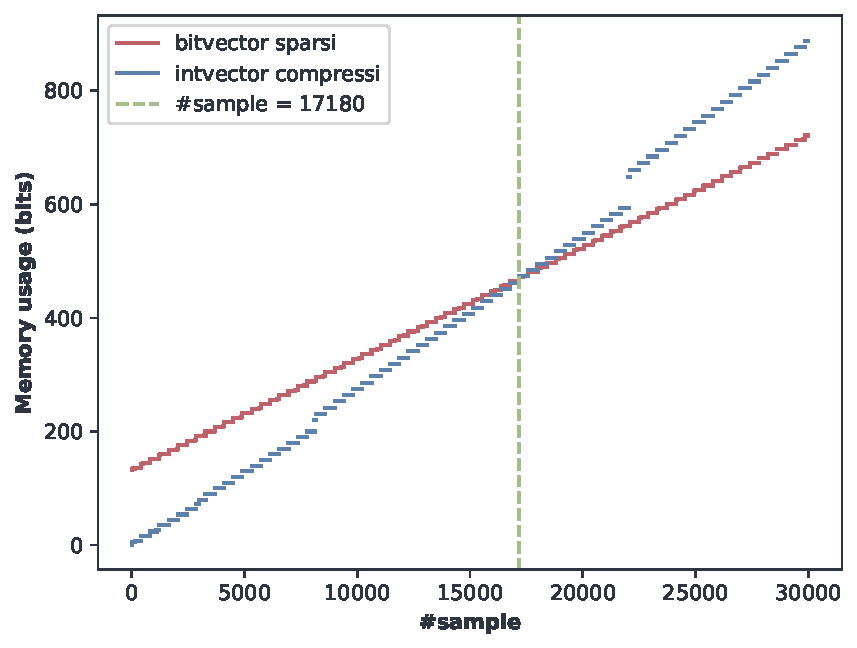
\includegraphics[scale = 0.7]{img/bv_vs_iv.pdf}
  \caption{Confronto tra la stima di memoria in bit necessaria a un bitvector
    sparso e a un 
    intvector compresso, al variare dell'altezza del pannello. Con la linea
    verde si segnala il numero di sample dopo il quale si ha un vantaggio
    in memoria nell'usare un bitvector sparso.}
  \label{fig:bvvsint}
\end{figure}